\chapter{Vectores normales y su uso}
Un vector normal es un vector que es perpendicular a un objeto concreto. En el caso tridimensional, un vector normal (o simplemente, normal) a una superfície es un vector perpendicular al plano tangente de aquella superfície. La normal es usada a menudo en motores gráficos para determinar la orientación de una superfície con respecto a una fuente de luz o a la cámara.
\begin{figure} [h!]
  \centering
  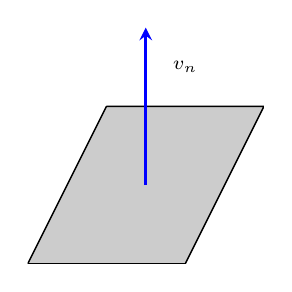
\begin{tikzpicture}
    \clip (0.5,0.5) rectangle (3.5, 3.5);
    \draw [-, line width=0.5pt, color=black]
    (0.5, 0.5) -- (2.5, 0.5)
    (2.5, 0.5) -- (3.5, 2.5)
    (3.5, 2.5) -- (1.5, 2.5)
    (1.5, 2.5) -- (0.5, 0.5);

    \draw [fill, color=black, opacity=0.2]
    (0.5, 0.5) -- (2.5, 0.5) -- (3.5, 2.5) -- (1.5, 2.5);

    \draw [->, >=stealth , line width=1pt, color=blue]
    (2, 1.5) -- (2, 3.5);

    \begin{scriptsize}
      \draw[color=black] (2.5, 3) node {$v_n$};
      \end{scriptsize}
  \end{tikzpicture}
\end{figure}

\section {Transformación de vectores noramles en OpenGL}
Cuando la iluminación es activada en OpenGL, los vectores normales son usados para determinar cuanta luz es recibida en el vértice o superfície especificado. Este procesado ocurre en el espacio de coordenadas de vista, por lo tanto, los vectores normales también son transformados por la matriz GL\_MODELVIEW.
Sin embargo, los vectores normales son transformados en una forma diferente de como lo hacen los vértices. No se puede simplemente multiplicar la matriz GL\_MODELVIEW y la normal.

Para entender cómo se transforman los vectores normales, hay que pensar en las normales como en coeficientes de ecuaciones del plano, que son perpendiculares a los planos.

Imaginemos un triangulo con tres vértices; ($v_1$, $v_2$, $v_3$), y la normal de esta superfície es $\vec{n} = (n_x, n_y, n_z, n_w)$. Si pensamos en el triangulo como un plano homogéneo, la ecuación del plano se vuelve: $n_xx + n_yy + n_zz + n_ww = 0$

Puesto que hay tres vértices en este plano, la ecuación del plano también se cumple cuando se sustituyen estos vértices en la ecuación. Por ejemplo, para $v_1 = (x_1,y_1,z_1,w_1)$, se cumple; $n_xx_1 + n_yy_1+n_zz_1+n_ww_1=0$
La forma en matriz de la ecuación del plano es la siguiente;
\[
\begin{pmatrix}
  n_x && n_y && n_z && n_w
\end{pmatrix}
\begin{pmatrix}
  x \\ y \\ z \\ w
\end{pmatrix}
= 0
\]

La ecuación del plano se consigue multiplicando la normal transpuesta y el vértice.
Ahora, modificamos la ecuación anterior para adquirir la formula de tranformación de vectores normales insertando las matrices M (GL\_MODELVIEW) y $M^{-1}$ en medio; es importante recordad que la ecuación sigue siendo equivalente ya que la inversa de una matriz por la matriz original es igual a matriz identidad.
\[
\underbrace{\begin{pmatrix}
  n_x && n_y && n_z && n_w
\end{pmatrix}M^-1}_{normal}\underbrace{M
\begin{pmatrix}
  x \\ y \\ z \\ w
\end{pmatrix}}_{vertex}
= 0
\]

\begin{equation*}
  T \cdot P_i = P_f 
\end{equation*}
Dónde $T$ es la matriz de transformación (GL\_MODELVIEW), $P_i$ es el punto original y $P_f$ es el punto final.

A continuación se eneñarán los tres tipos de transformaciones (explicadas en el capítulo anterior) que se pueden aplicar a los puntos y cuáles son las que afectan a las normales. 

\subsection{Translación}
En las siguientes figuras se puede observar que después de aplicar un movimiento de translación, el mó
\begin{minipage}{0.5\textwidth}
  \centering
  \begin{tikzpicture}
    \clip (0, 0) rectangle (4, 5)
    (0.5,1) node (1) {}
    (2,1) node (2){}
    (2,2.5) node (3){}
    (0.5,2.5) node (4){}
    (1,3) node (5){}
    (2.5,3) node (6){}
    (2.5,1.5) node (7){}
    (2.25,2) node (8){}
    (3,2) node (9){}
    (3.5,1.5) node (10){}
    (1,4) node (11){}
    (1.5,3.5) node (12){}
    (0,0.5) node (13){}
    (1.5, 2.75) node (14) {};

    \draw[-, color=black]
    (1.center) -- (2.center) -- (3.center) -- (4.center) -- (1.center)
    (4.center) -- (5.center)
    (3.center) -- (6.center)
    (5.center) -- (6.center)
    (6.center) -- (7.center)
    (7.center) -- (2.center);

    \draw[->, color=black, >=stealth]
    (1.center) -- (13.center);
    \draw[->, color=black, >=stealth]
    (7.center) -- (10.center);
    \draw[->, color=black, >=stealth]
    (5.center) -- (11.center);

    \draw[->, >=latex, color=red]
    (8.center) -- (9.center);
    \draw[->, >=latex, color=blue]
    (14.center) -- (12.center);

  \end{tikzpicture}

  
\end{minipage}
\begin{minipage}{0.5\textwidth}
  \centering
  \begin{tikzpicture}
    \clip (0,0) rectangle (4,5)
    (1.5,1) node (1) {}
    (3,1) node (2) {}
    (3,2.5) node (3) {}
    (1.5,2.5) node (4) {}
    (2,3) node (5) {}
    (3.5,3) node (6) {}
    (3.5,1.5) node (7) {}
    (3.25,2) node (8) {}
    (4,2) node (9) {}
    (2.5,3.5) node (10) {}
    (1,4) node (11) {}
    (0,0.5) node (12) {}
    (1,1.5) node (13) {}
    (1.5,1.5) node (14) {}
    (2.5, 2.75) node (15) {};

    \draw[-, color=black]
    (1.center) -- (2.center) -- (3.center) -- (4.center) -- (1.center)
    (4.center) -- (5.center)
    (5.center) -- (6.center)
    (6.center) -- (7.center)
    (7.center) -- (2.center)
    (3.center) -- (6.center)
    (13.center) -- (14.center);

    \draw[->, >=stealth]
    (13.center) -- (12.center);
    \draw[->, >=stealth]
    (13.center) -- (11.center);

    \draw[->, >=latex, color=blue]
    (15.center) -- (10.center);
    \draw[->, >=latex, color=red]
    (8.center) -- (9.center);
  \end{tikzpicture}
\end{minipage}

